\documentclass[letterpaper]{article}
\usepackage{typearea}
\typearea{12}
\usepackage{here}
\usepackage{bm}
\usepackage{amsmath, amsfonts}
\usepackage[top=20truemm,bottom=20truemm,left=25truemm,right=25truemm]{geometry}
\usepackage[dvipdfmx]{hyperref,graphicx}

\begin{document}
\title{The Art of Linear Algebra\\
\vspace{5pt}
\large{
-- Graphic Notes on ``Linear Algebra for Everyone" --
}
}

\author{Kenji Hiranabe
\thanks{twitter: @hiranabe, k-hiranabe@esm.co.jp, \url{https://anagileway.com}} \\
with the kindest help of Gilbert Strang
\thanks{Massachusetts Institute of Technology, \url{http://www-math.mit.edu/\~gs/}}
}

\date{\today}

\maketitle

\vspace{-5pt}
 
\begin{abstract}
I tried intuitive visualizations of important concepts introduced
in ``Linear Algebra for Everyone".\footnote{``Linear Algebra for Everyone":
\url{http://math.mit.edu/everyone/} with Japanese translation started by Kindai Kagaku.}\linebreak
This is aimed at promoting understanding of vector/matrix calculations
and algorithms from the\linebreak perspectives of matrix factorizations.
They include Column-Row ($\bm{CR}$), Gaussian Elimination ($\bm{LU}$),
Gram-Schmidt Orthogonalization ($\bm{QR}$), Eigenvalues and Diagonalization ($\bm{Q \Lambda Q^\mathbf{T}}$),
and Singular Value Decomposition ($\bm{U \Sigma V^\mathbf{T}}$).
\end{abstract}

\section*{Foreword}
I am happy to see Kenji Hiranabe's pictures of matrix operations in linear algebra !
The pictures are an excellent way to show the algebra.  We can think of matrix
multiplications by row $\bm{\cdot}$ column dot products, but that is not all --  it is ``linear combinations"
and ``rank 1 matrices" that complete the algebra and the art.
I am very grateful to see the books in Japanese translation
and the ideas in Kenji's pictures.
\begin{flushright}
-- Gilbert Strang \\ Professor of Mathematics at MIT
\end{flushright}

\tableofcontents

\section{Viewing a Matrix -- 4 Ways}

A matrix ($m \times n$) can be seen as $1$ matrix, $mn$ numbers, $n$ columns and $m$ rows.

\begin{figure}[H]
  \centering
  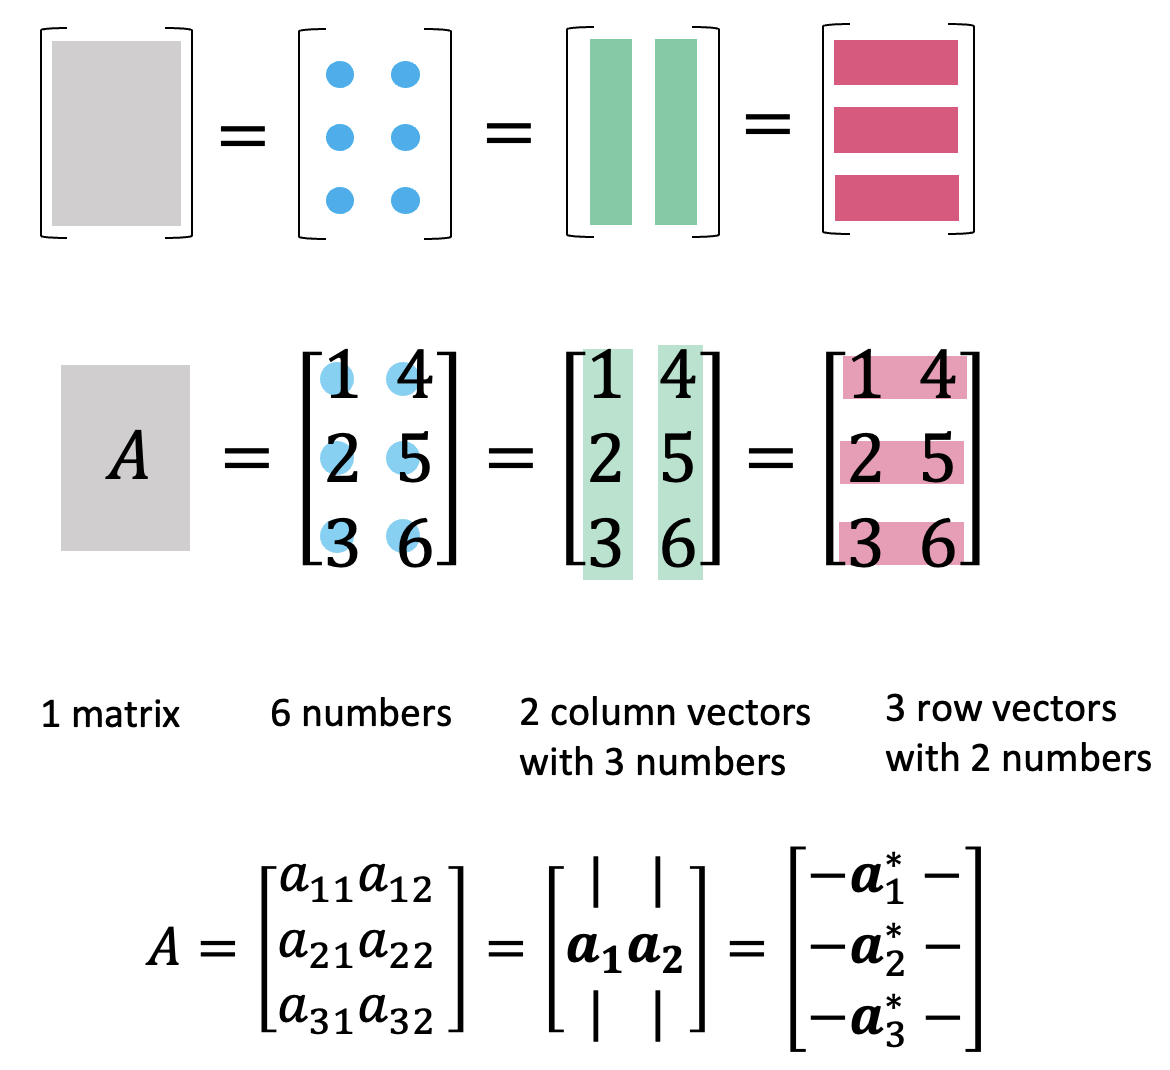
\includegraphics[keepaspectratio, width=7cm]{ViewingMatrix-4Ways.png}
  \caption{Viewing a Matrix in 4 Ways}
\end{figure}


\begin{equation*}
  A= \begin{bmatrix}
    a_{11} & a_{12}\\
    a_{21} & a_{22}\\
    a_{31} & a_{32}
  \end{bmatrix}
  =
  \begin{bmatrix}
    | & |\\
    \bm{a_1} & \bm{a_2}\\
    | & |
  \end{bmatrix}
  =
  \begin{bmatrix}
    - \bm{a_1^*} -\\
    - \bm{a_2^*} -\\
    - \bm{a_3^*} -
  \end{bmatrix}
\end{equation*} \\

Here, the column vectors are in bold as $\bm{a_1}$.
Row vectors include $\bm{*}$ as in $\bm{a_1^*}$.
Transposed vectors and matrices are indicated by $\mathrm{T}$ as
in $\bm{a}^{\mathrm{T}}$ and $A^{\mathrm{T}}$.


\section{Vector times Vector -- 2 Ways}

Hereafter I point to specific sections of ``Linear Algebra for Everyone" 
and present graphics which illustrate the concepts with short names
in colored circles.

\begin{itemize}
  \item Sec. 1.1 (p.2) Linear combination and dot products
  \item Sec. 1.3 (p.25) Matrix of Rank One
  \item Sec. 1.4 (p.29) Row way and column way
\end{itemize} 


\begin{figure}[H]
  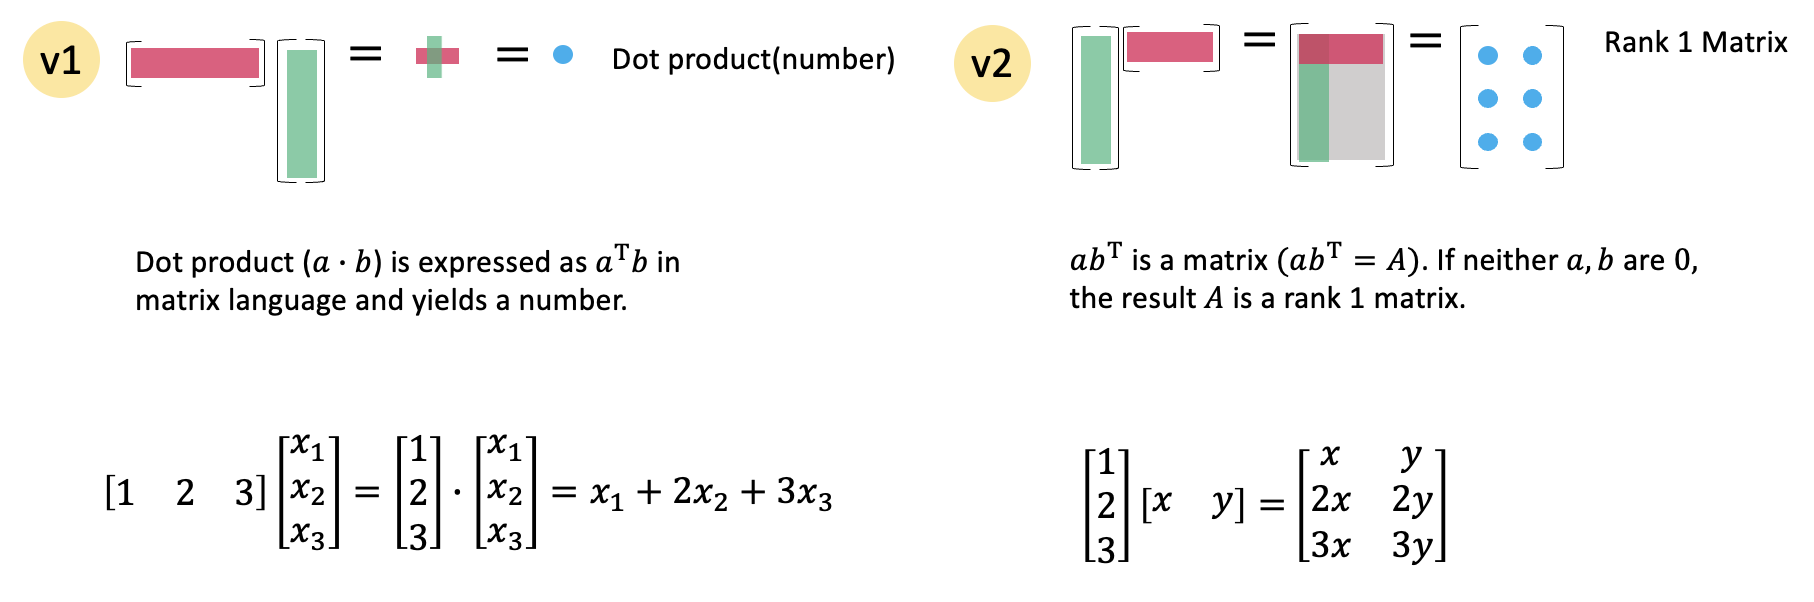
\includegraphics[keepaspectratio, width=\linewidth]{VectorTimesVector.png}
  \caption{Vector times Vector - (v1), (v2)}
\end{figure}

\section{Matrix times Vector -- 2 Ways}

A matrix times a vector creates a vector of three dot products (Mv1)
as well as a linear combination (Mv2) of the column vectors of $A$.

\begin{itemize}
  \item Sec. 1.1 (p.3) Linear combinations
  \item Sec. 1.3 (p.21) Matrices and Column Spaces
\end{itemize} 

\begin{figure}[H]
  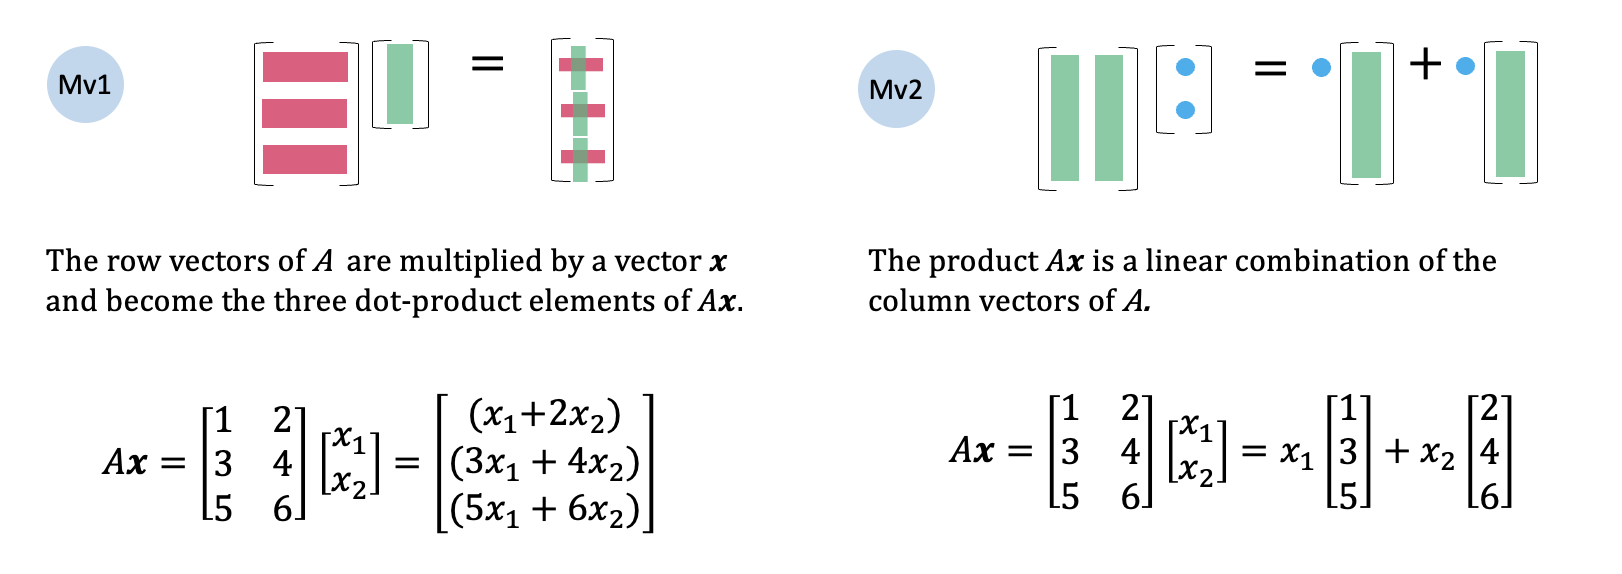
\includegraphics[keepaspectratio, width=\linewidth]{MatrixTimesVector.png}
  \caption{Matrix times Vector - (Mv1), (Mv2)}
\end{figure}

At first, you learn (Mv1). But when you get used to viewing it as (Mv2),
you can understand $Ax$ as a linear combination of the columns of $A$.
Those products fill the column space of $A$  denoted as $\mathbf{C}(A)$.
The solution space of $Ax=0$ is the nullspace of $A$ denoted as $\mathbf{N}(A)$.

The four subspaces consists of $\mathbf{N}(A)$ + $\mathbf{C}(A^\mathbf{T})$ 
(which are perpendicular to each other) in $\mathbb{R}^n$ and
$\mathbf{N}(A^\mathbf{T})$ + $\mathbf{N}(A)$ in $\mathbb{R}^m$
(which are perpendicular to each other).

\begin{itemize}
  \item Sec. 3.5 (p.124) Dimentions of the Four Subspaces
\end{itemize} 

\begin{figure}[H]
  \centering
  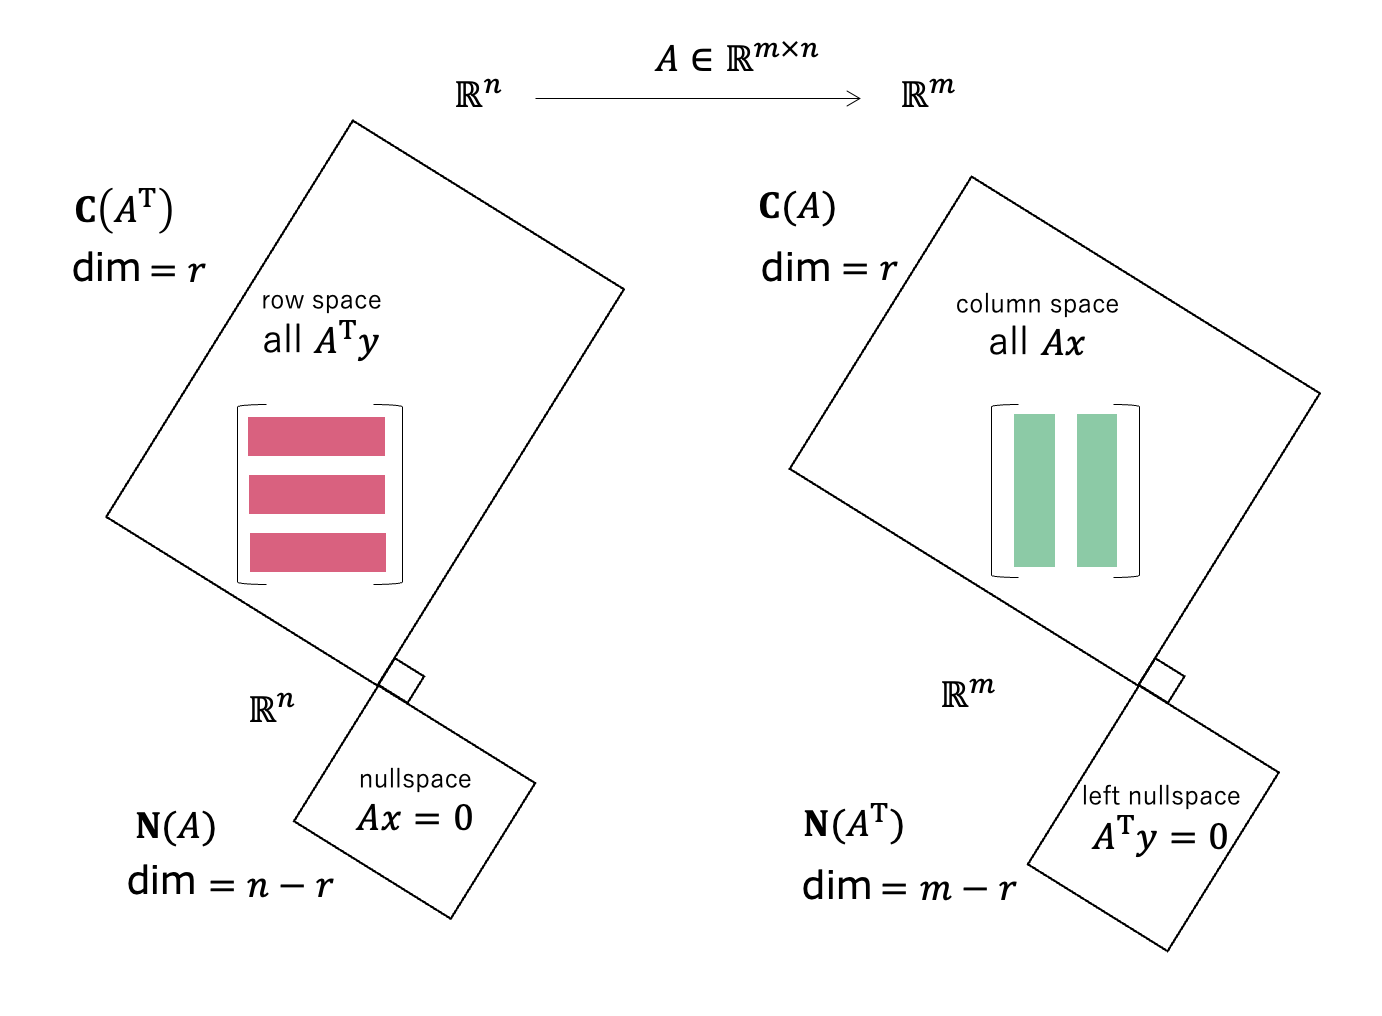
\includegraphics[keepaspectratio, width=8cm]{4-Subspaces.png}
  \caption{The Four Subspaces}
\end{figure}

See $A=CR$ (Sec 6.1) for the rank $r$.


\clearpage

\section{Matrix times Matrix -- 4 Ways}

``Matrix times Vector" naturally extends to ``Matrix times Matrix".

\begin{itemize}
  \item Sec. 1.4 (p.35) Four Ways to Multiply $\bm{AB=C}$
  \item Also see the back cover of the book
\end{itemize} 


\begin{figure}[H]
  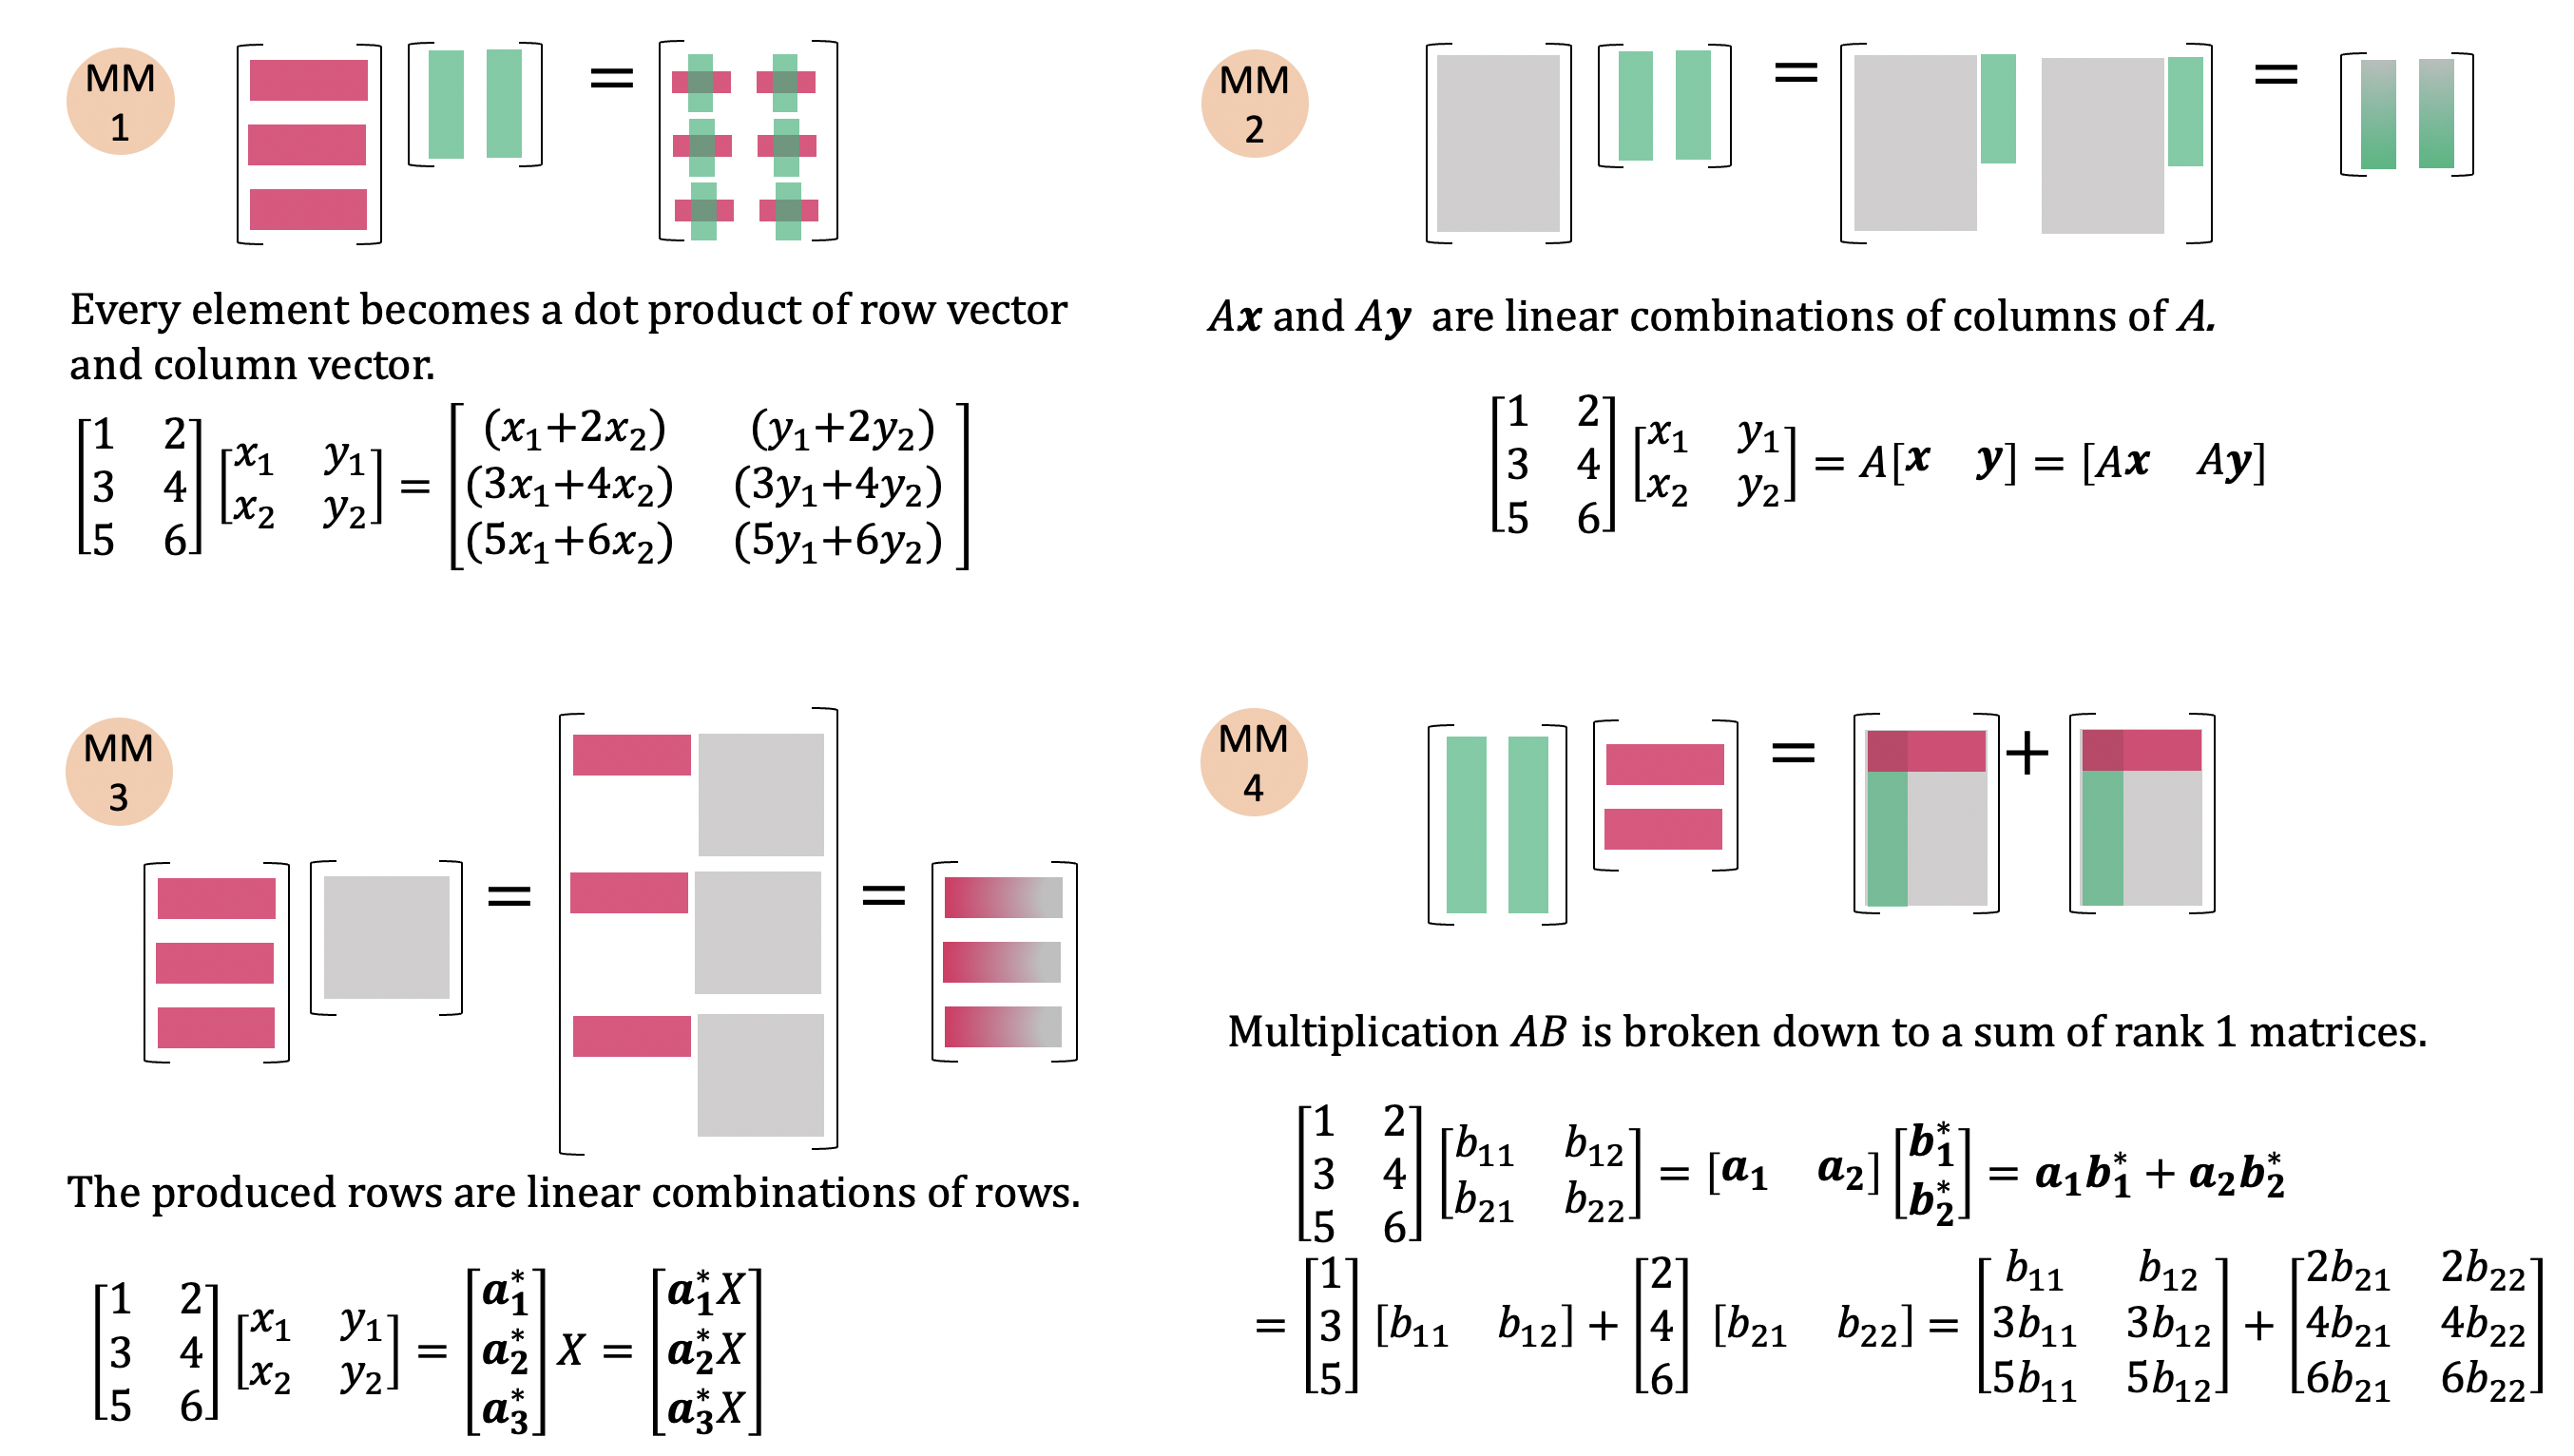
\includegraphics[keepaspectratio, width=\linewidth]{MatrixTimesMatrix.png}
  \caption{Matrix times Matrix - (MM1), (MM2), (MM3), (MM4)}
\end{figure}

\clearpage


\section{Practical Patterns}

Here, I show some practical patterns which allow you to capture
the coming factorizations more intuitively.

\begin{figure}[H]
  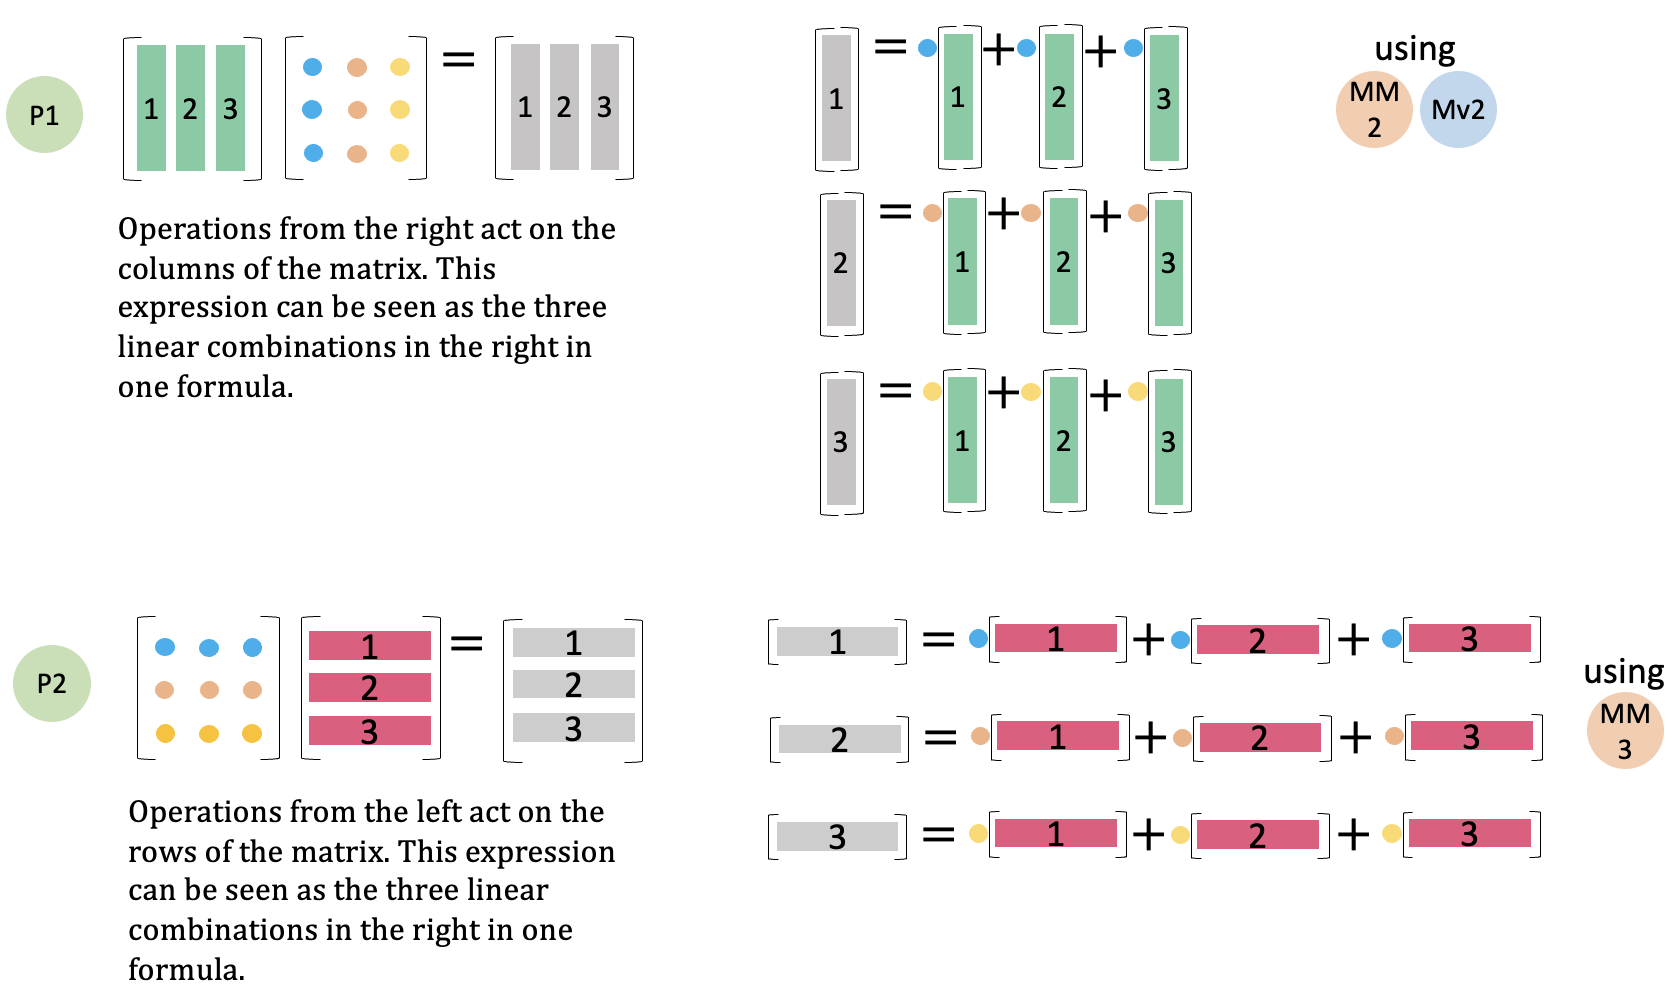
\includegraphics[keepaspectratio, width=\linewidth]{Pattern12.png}
  \caption{Pattern 1, 2 - (P1), (P1)}
\end{figure}

Pattern 1 is a combination of (MM2) and (Mv2).
Pattern 2 is an extention of (MM3). Note that Pattern 1 is a column operation (multiplying a matrix from right),
whereas Pattern 2 is a row operation (multiplying a matrix from left).

\begin{figure}[H]
  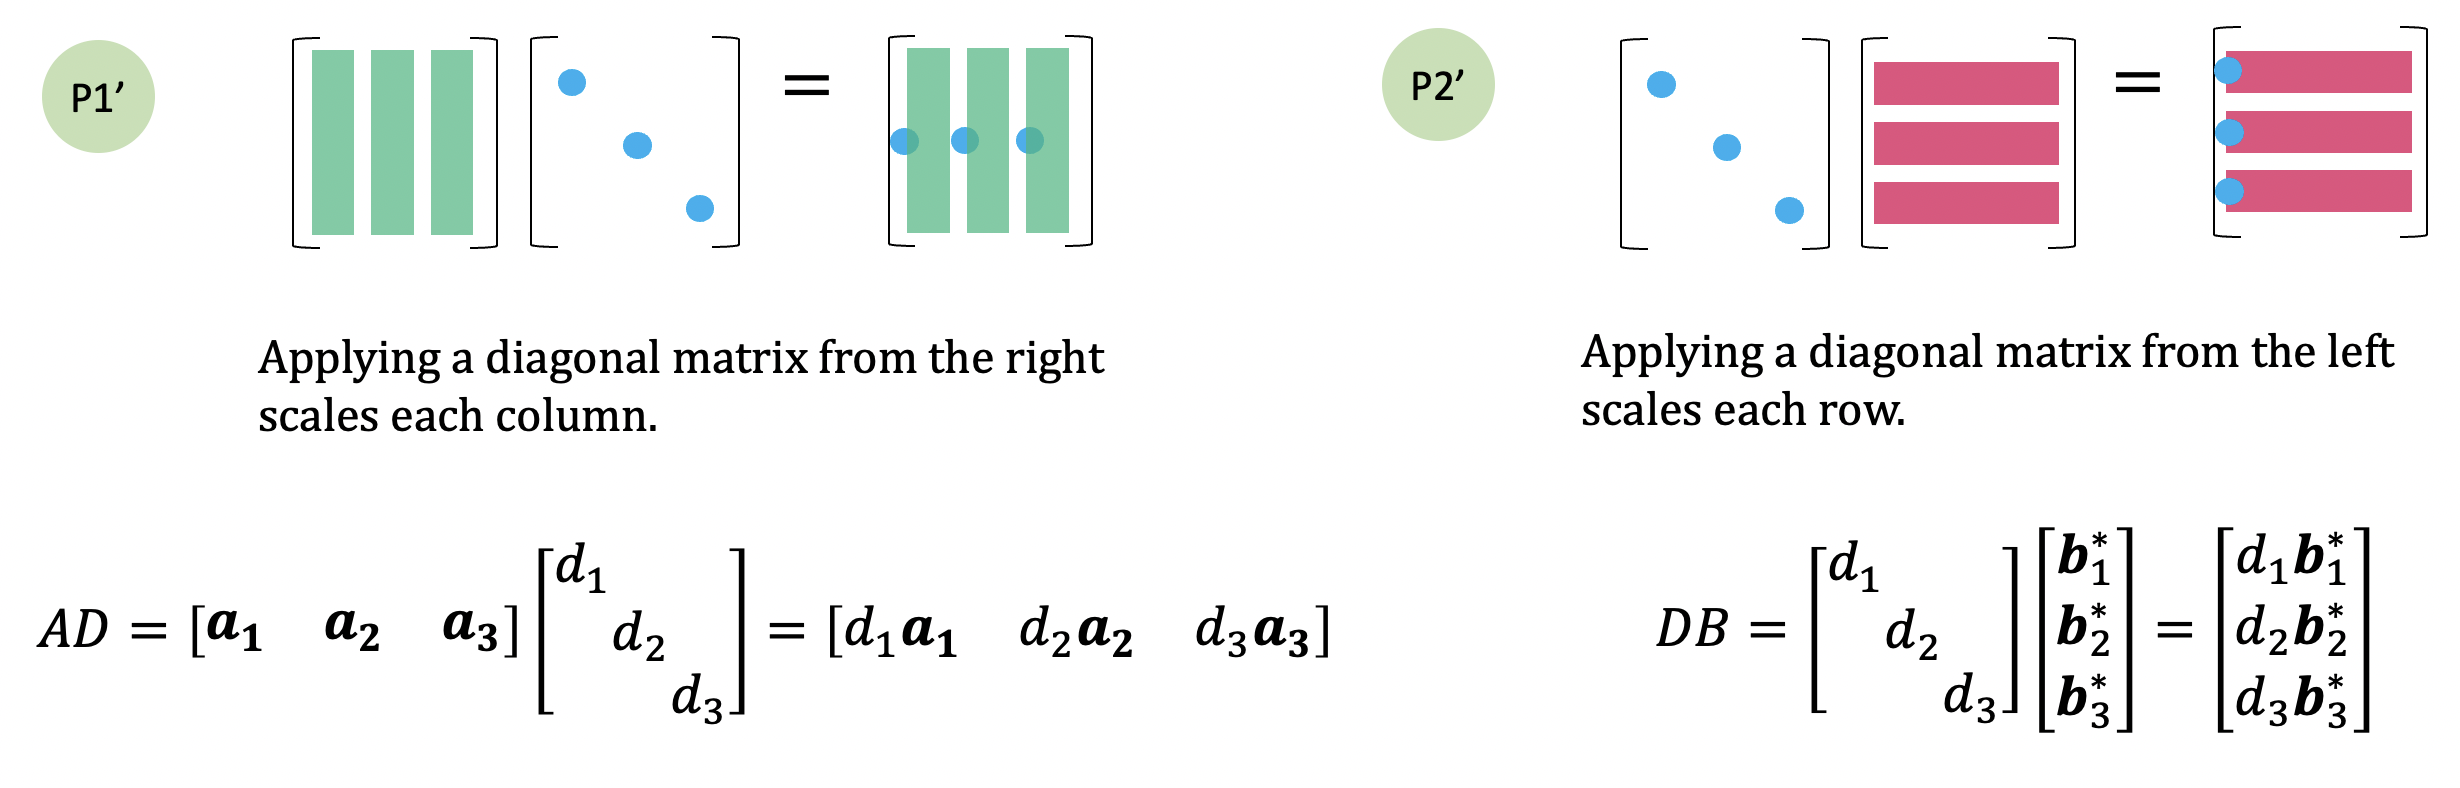
\includegraphics[keepaspectratio, width=\linewidth]{Pattern11-22.png}
  \caption{Pattern 1$^\prime$, 2$^\prime$ - (P1$^\prime$), (P2$^\prime$)}
\end{figure}

(P1$^\prime$) multipies the diagonal numbers to the columns of the matrix,
whereas (P2$^\prime$) multipies the diagonal numbers to the row of the matrx.
Both are variants of (P1) and (P2).

\begin{figure}[H]
  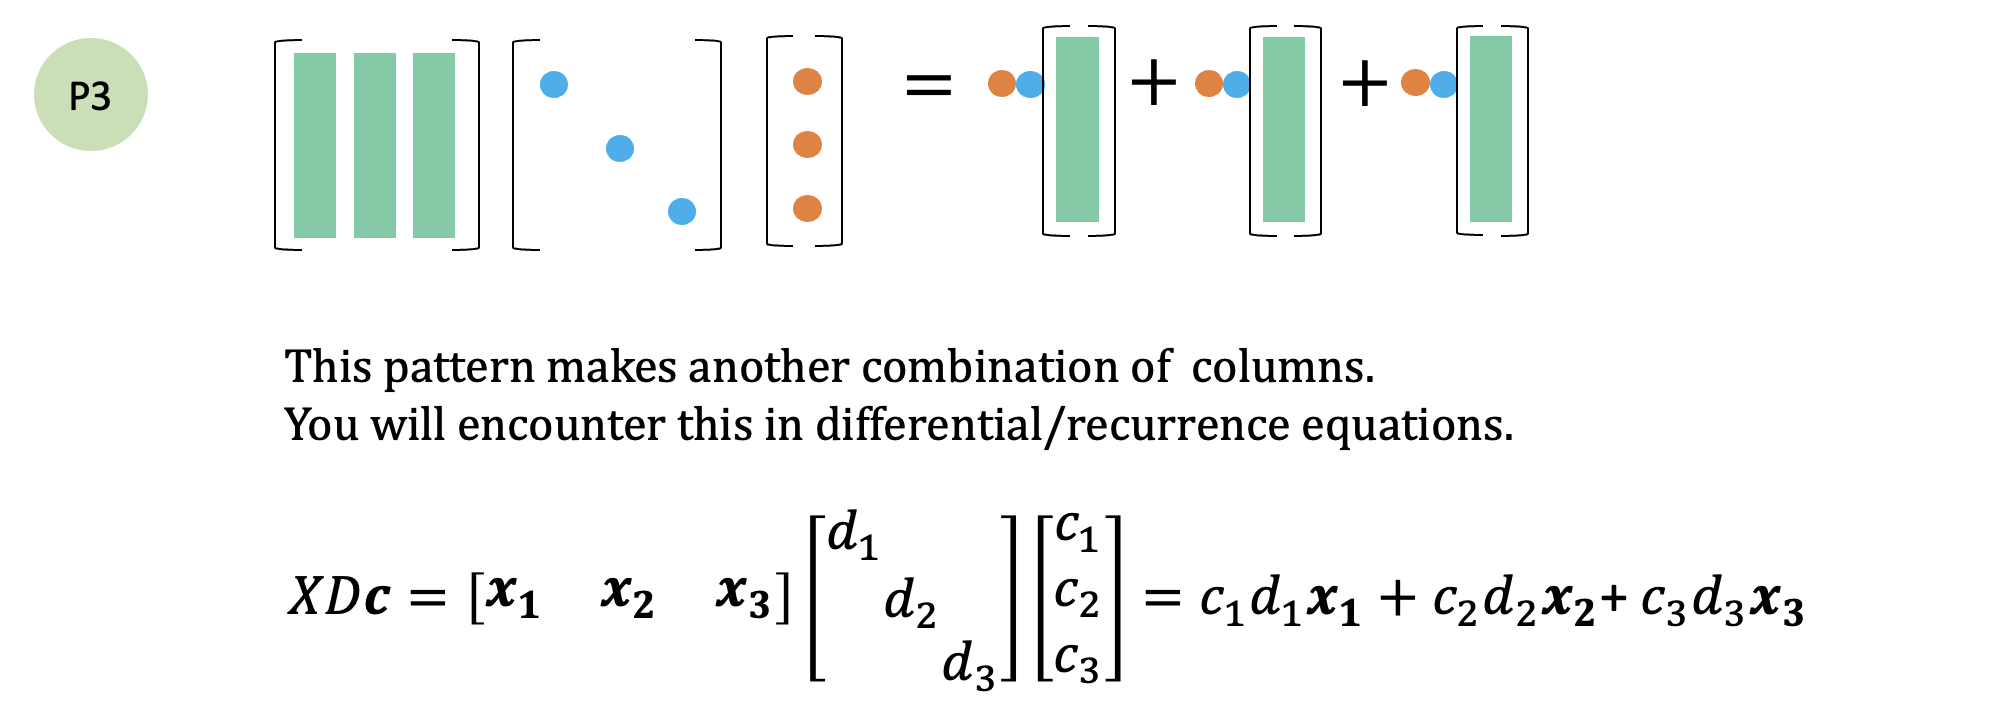
\includegraphics[keepaspectratio, width=\linewidth]{Pattern3.png}
  \caption{Pattern 3 - (P3)}
\end{figure}

This pattern appears when you solve differential equations and recurrence equations:

\begin{itemize}
  \item Sec. 6 (p.201) Eigenvalues and Eigenvectors
  \item Sec. 6.4 (p.243) Systems of Differential Equations
\end{itemize} 

\begin{align*}
  \frac{d \bm{u}(t) }{dt} &= A \bm{u}(t), \quad \bm{u}(0)=\bm{u}_0\\
  \bm{u}_{n+1} &= A \bm{u}_n, \quad \bm{u_0} = \bm{u}_0
\end{align*}

In both cases, the solutions are expressed with
eigenvalues ($\lambda_1, \lambda_2, \lambda_3$), 
eigenvectors $X=\begin{bmatrix} \bm{x}_1 & \bm{x}_2 & \bm{x}_3 \end{bmatrix}$ of $A$, and
the coefficients $c=\begin{bmatrix} c_1 & c_2 & c_3 \end{bmatrix}^\mathbf{T}$
which are the coordinates of the initial condition $\bm{u}(0)=\bm{u}_0$ in terms of
the eigenvectors $X$.

\begin{equation*}
  \bm{u}_0 = c_1 \bm{x}_1 + c_2 \bm{x}_2 + c_3 \bm{x}_3
\end{equation*}
\begin{equation*}
  \bm{c} =
  \begin{bmatrix}
    c_1\\
    c_2\\
    c_3
  \end{bmatrix} = X^{-1} \bm{u}_0
\end{equation*}

and the general solution of the two equations are:

\begin{align*}
  \bm{u}(t) &= e^{At} \bm{x}_0 &= X e^{\Lambda t} \bm{c} &= c_1 e^{\lambda_1 t} \bm{x}_1 + c_2 e^{\lambda_2 t} \bm{x}_2 + c_3 e^{\lambda_3 t} \bm{x}_3\\
  \bm{u}_n &= A^n \bm{x}_0 &= X \Lambda^n \bm{c} &= c_1 \lambda_1^n \bm{x}_1 + c_2 \lambda_2^n \bm{x}_2 + c_3 \lambda_3^n \bm{x}_3
\end{align*}

See Figure 9: Pattern 3 (P3) above again for $XDc$.

\begin{figure}[H]
  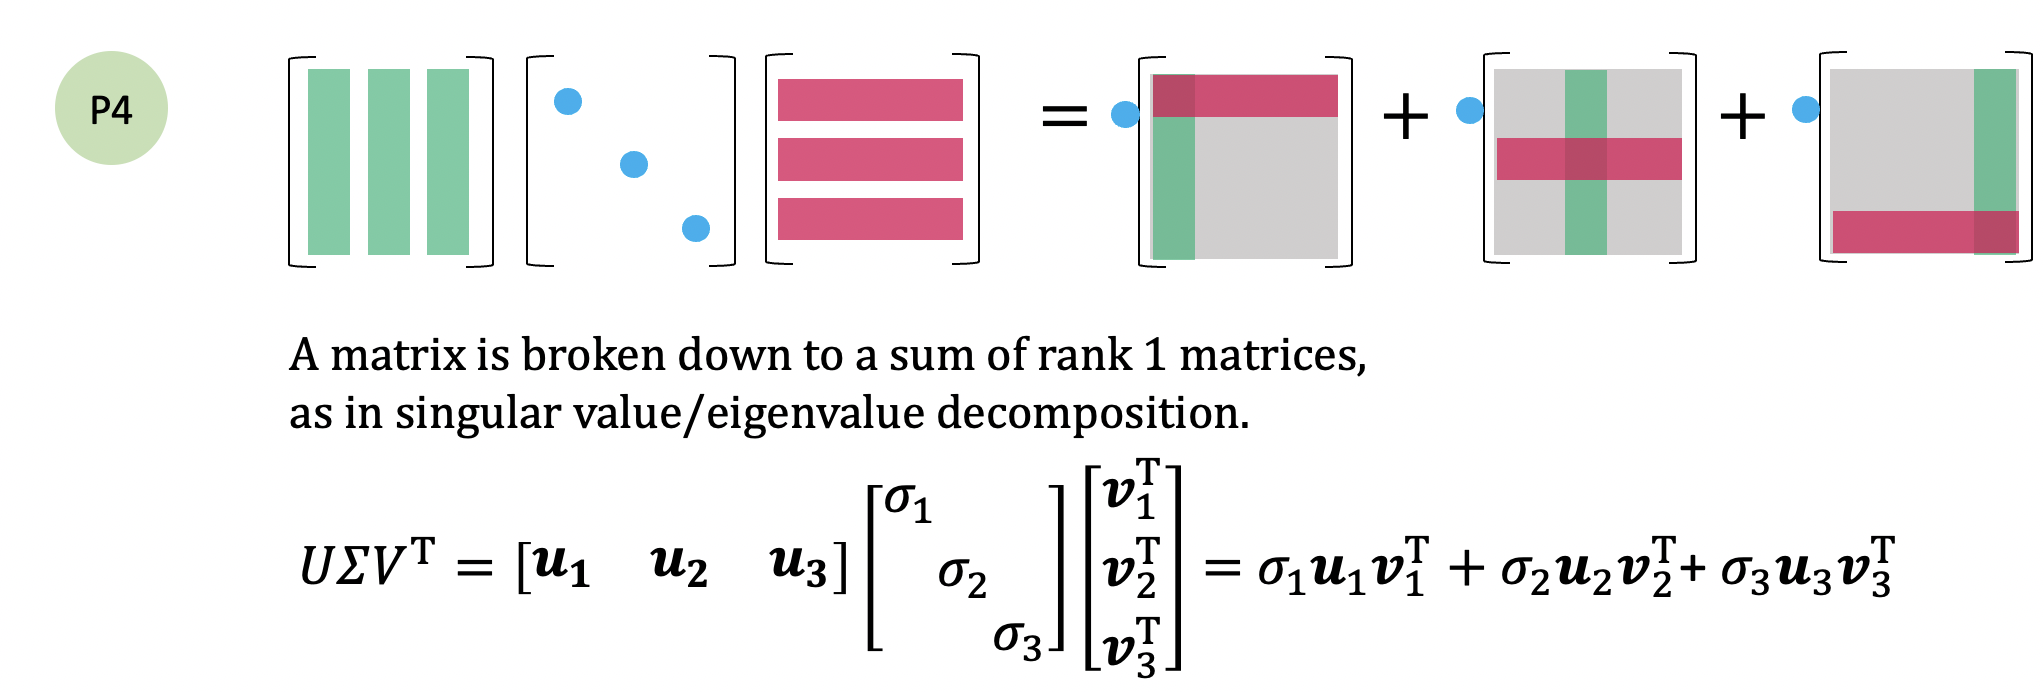
\includegraphics[keepaspectratio, width=\linewidth]{Pattern4.png}
  \caption{Pattern 4 - (P4)}
\end{figure}

This pattern (P4) works in both eigenvalue decomposition and singular value decomposition.
Both decompositions are expressed as a product of three matrices with a diagonal matrix in the middle,
and also a sum of rank 1 matrices with the eigenvalue/singular value coefficients.

More details are discussed in the next section.

\clearpage

\section{The Five Factorizations of a Matrix}

\begin{itemize}
  \item Preface p.vii, The Plan for the Book.
\end{itemize}
$A=CR, A=LU, A=QR, A=Q \Lambda Q^\mathbf{T}\, A=U \Sigma V^\mathbf{T}$ are 
illustrated one by one.

\begin{figure}[H]
  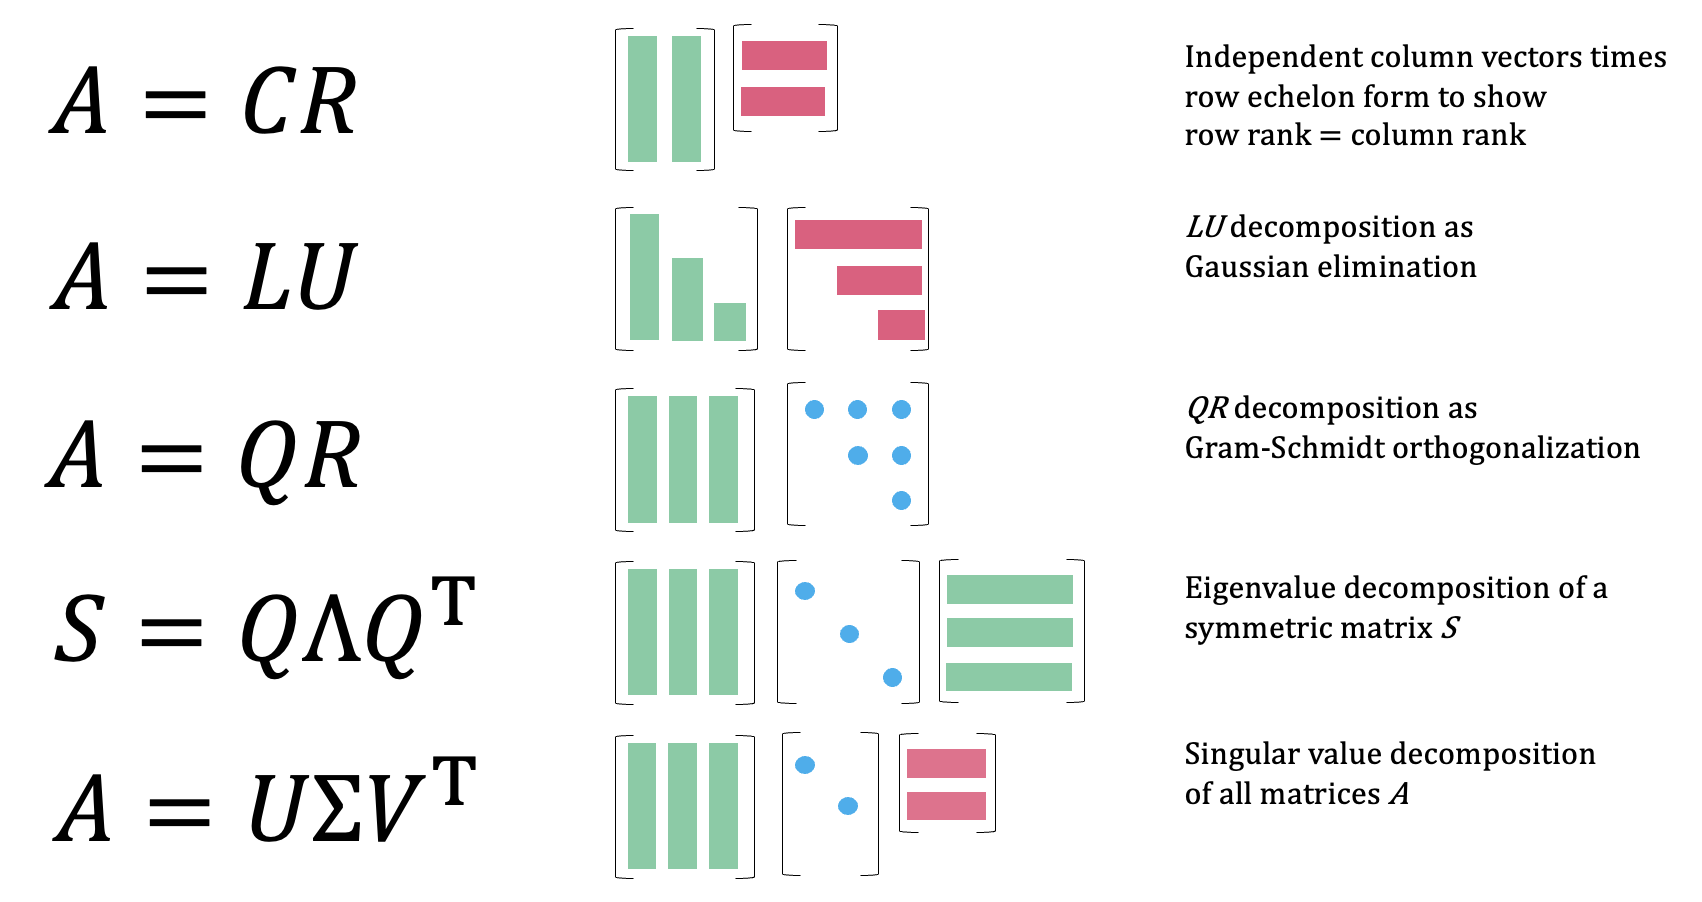
\includegraphics[keepaspectratio, width=\linewidth]{5-Factorizations.png}
  \caption{The Five Factorizations}
\end{figure}

\clearpage

\subsection{$\boldsymbol{A=CR}$}

\begin{itemize}
  \item Sec.1.4 Matrix Multiplication and $\bm{A=CR}$ (p.29)
\end{itemize}

All general rectangular matrices $A$ have the same row rank as the column rank.
This factorization is the most intuitive way to understand this theorem.
$C$ consists of independent columns of $A$, and $R$ is the row reduced echelon form of $A$.
$A=CR$ reduces to $r$ independent columns in $C$ times $r$ independent rows in $R$.

\begin{equation*}
  \begin{split}
    A &= CR\\
  \begin{bmatrix}
    1 & 2 & 3 \\
    2 & 3 & 5
  \end{bmatrix}
  & =
  \begin{bmatrix}
    1 & 2 \\
    2 & 3
  \end{bmatrix}
  \begin{bmatrix}
    1 & 0 & 1 \\
    0 & 1 & 1
  \end{bmatrix}
\end{split}
\end{equation*}

Procedure: Look at the columns of $A$ from left to right. Keep independent ones,
discard dependent ones which can be created by the former columns.
The column 1 and the column 2 survive, and the column 3 is discarded
because it is expressed as a sum of the former two columns.
To rebuild $A$ by the independent columns 1, 2, you find a row echelon form $R$
appearing in the right.

\begin{figure}[H]
  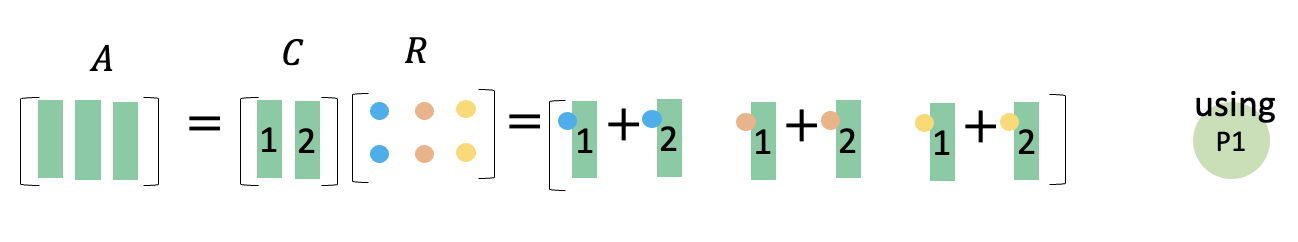
\includegraphics[keepaspectratio, width=\linewidth]{CR1.png}
  \caption{Column Rank in $CR$}
\end{figure}

Now you see the column rank is two because there are only two independent columns in $C$
and all the columns of $A$ are linear combinations of the two columns of $C$.

\begin{figure}[H]
  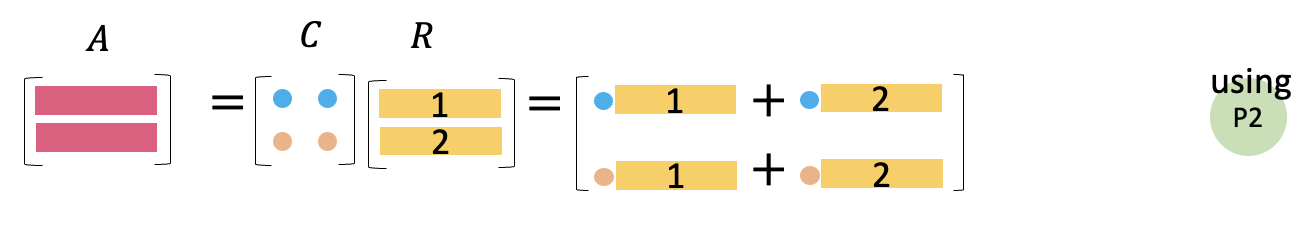
\includegraphics[keepaspectratio, width=\linewidth]{CR2.png}
  \caption{Row Rank in $CR$}
\end{figure}

And you see the row rank is two because there are only two independent rows in $R$
and all the rows of $A$ are linear combinations of the two rows of $R$.

\clearpage

\subsection{$\boldsymbol{A=LU}$}

Solving $Ax=b$  via Gaussian elimination can be expressed as a $LU$ factorization.
Usually, you apply elementary row operation matrices ($E$) from left of $A$ to make upper trianglar $U$.

\begin{align*}
  EA &= U\\
  A &= E^{-1}U\\
\text{let} \; L = E^{-1}, \quad  A &= LU
\end{align*}

Now solve $Ax=b$ in 2 steps: 1) forward $Lc=b$ and 2) back $Ux=c$.


\begin{itemize}
  \item Sec.2.3 (p.57) Matrix Computations and $\bm{A=LU}$
\end{itemize}

Here, we directly calculate $L$ and $U$ from $A$.

\begin{equation*}
  A = 
      \begin{bmatrix}
        |\\
        \bm{l}_1\\
        |
      \end{bmatrix}
      \begin{bmatrix}
        -  \bm{u}^*_1  -
      \end{bmatrix}
  +  \begin{bmatrix}
      0 & \begin{matrix} 0 & 0 \end{matrix}\\
      \begin{matrix} 0 \\ 0 \end{matrix} & A_2
    \end{bmatrix}
  = 
  \begin{bmatrix}
    |\\
    \bm{l}_1\\
    |
  \end{bmatrix}
  \begin{bmatrix}
    - \bm{u}^*_1 -
  \end{bmatrix}
  +
  \begin{bmatrix}
    |\\
    \bm{l}_2\\
    |
  \end{bmatrix}
  \begin{bmatrix}
    - \bm{u}^*_2  -
  \end{bmatrix}
  +  \begin{bmatrix}
  0 & 0 & 0\\
  0 & 0 & 0 \\
  0 & 0 & A_3
  \end{bmatrix} = LU
\end{equation*}
 

\begin{figure}[H]
  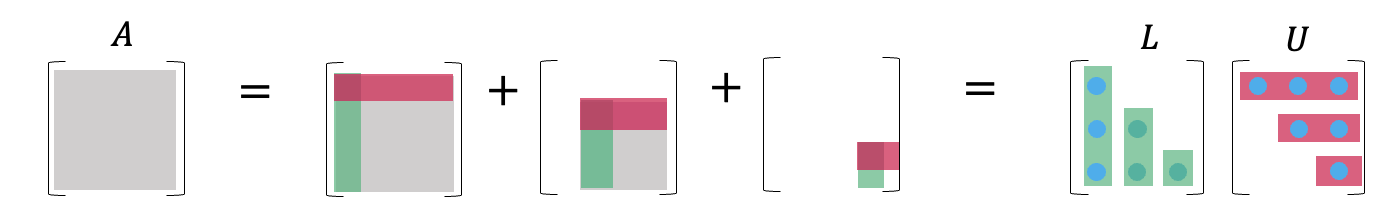
\includegraphics[keepaspectratio, width=\linewidth]{LU1.png}
\caption{Recursive Rank 1 Matrix Peeling from $A$}
\end{figure}

To find $L$ and $U$, peel off the rank 1 matrix made of
the first row and the first column of $A$.
This leaves $A_2$. Do this recursively and decompose $A$ into the sum of rank 1 matrices.


\begin{figure}[H]
  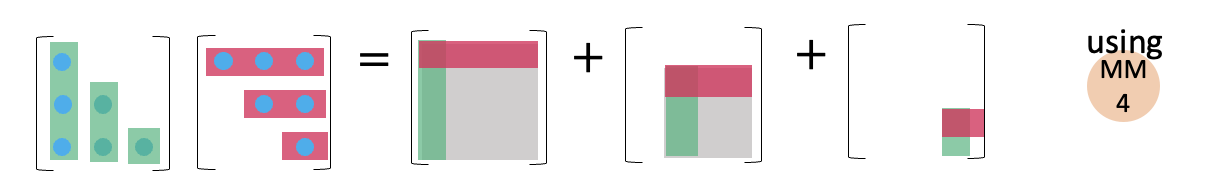
\includegraphics[keepaspectratio, width=\linewidth]{LU2.png}
\caption{$LU$ rebuilds $A$}
\end{figure}

To rebuild $A$ from $L$ times $U$ is easy.

\clearpage

\subsection{$\boldsymbol{A=QR}$}

$A=QR$ changes the columns of $A$ into perpendicular columns of $Q$, keeping $\bm{C}(A) = \bm{C}(Q)$.

\begin{itemize}
  \item Sec.4.4 Orthogonal matrices and Gram-Schmidt (p.165)
\end{itemize}

In Gram-Schmidt, the normalized $\bm{a}_1$ is picked up as $\bm{q}_1$ first and then
$\bm{a}_2$ is adjusted to be perpendicular to $\bm{q}_1$ to create $\bm{q}_2$, and this
procedure goes on.

\begin{align*}
  \bm{q}_1 &= \bm{a}_1/|\bm{a}_1| \\
  \bm{q}_2 &= \bm{a}_2 - \bm{q}_1^\mathbf{T} \bm{a}_2, \quad \bm{q}_2 = \bm{q}_2/|\bm{q}_2| \\
  \bm{q}_3 &= \bm{a}_3 - \bm{q}_1^\mathbf{T} \bm{a}_3 - \bm{q}_2^\mathbf{T} \bm{a}_3, \quad \bm{q}_3 = \bm{q}_3/|\bm{q}_3|
\end{align*}

or you can write:

\begin{align*}
  \bm{a}_1 &= r_{11}\bm{q}_1\\
  \bm{a}_2 &= r_{12}\bm{q}_1 + r_{22} \bm{q}_2\\
  \bm{a}_3 &= r_{13}\bm{q}_1 + r_{23} \bm{q}_2 + r_{33} \bm{q}_3
\end{align*}

The original $A$ becomes $QR$: orthogonal times triangular.

\begin{gather*}
  A = 
  \begin{bmatrix}
    | & | & |\\
    \bm{q}_1 & \bm{q}_2 & \bm{q}_3\\
    | & | & |
  \end{bmatrix}
  \begin{bmatrix}
    r_{11} & r_{12} & r_{13}\\
           & r_{22} & r_{23}\\
           &        & r_{33}
  \end{bmatrix} = QR\\
  \\
  Q Q^\mathbf{T}=Q^\mathbf{T} Q = I
\end{gather*}

\begin{figure}[H]
  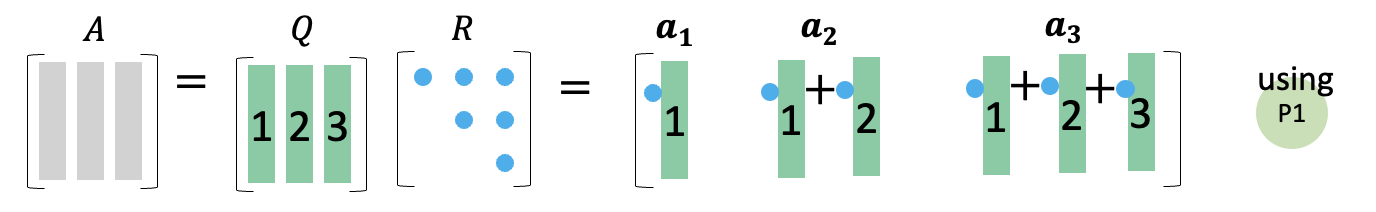
\includegraphics[keepaspectratio, width=\linewidth]{QR.png}
  \caption{$A=QR$}
\end{figure}

The column vectors of $A$ can be adjusted into an orthonormal set: the column vectors of $Q$.
Each column vector of $A$ can be rebuilt from $Q$ and the upper triangular matrix $R$ .

See Pattern 1 (P1) again for the graphic interpretation.


\clearpage

\subsection{$\boldsymbol{S=Q \Lambda Q^\mathbf{T}}$}

All symmetric matrices $S$ must have real eigenvalues and orthogonal eigenvectors.
The eigenvalues are the diagonal elementes of $\Lambda$ and the eigenvectors are in $Q$. 

\begin{itemize}
  \item Sec.6.3 (p.227) Symemtric Positive Definite Matrices
\end{itemize}

\begin{align*}
  S = Q \Lambda Q^\mathbf{T}
&= \begin{bmatrix}
    | & | & |\\
    \bm{q}_1 & \bm{q}_2 & \bm{q}_3\\
    | & | & |
  \end{bmatrix}
  \begin{bmatrix}
    \lambda_1 \\
           & \lambda_2 & \\
           & & \lambda_3
  \end{bmatrix}
  \begin{bmatrix}
  - \bm{q}_1^\mathbf{T} -\\
  - \bm{q}_2^\mathbf{T} -\\
  - \bm{q}_3^\mathbf{T} -
  \end{bmatrix}\\
  \\
  &=
  \lambda_1 \begin{bmatrix}
    |\\
    \bm{q}_1\\
    |
  \end{bmatrix}
  \begin{bmatrix}
    - \bm{q}_1^\mathbf{T} - 
  \end{bmatrix}
  +
  \lambda_2 \begin{bmatrix}
  |\\
  \bm{q}_2\\
  |
  \end{bmatrix}
  \begin{bmatrix}
  - \bm{q}_2^\mathbf{T} -
  \end{bmatrix} 
  +
  \lambda_3 \begin{bmatrix}
    |\\
    \bm{q}_3 \\
    |
  \end{bmatrix}
  \begin{bmatrix}
    - \bm{q}_3^\mathbf{T} -
  \end{bmatrix} \\
&= \lambda_1 P_1 + \lambda_2 P_2 + \lambda_3 P_3
\end{align*}

\begin{equation*}
  P_1=\bm{q}_1 \bm{q}_1^\mathbf{T}, \quad P_2=\bm{q}_2 \bm{q}_2^\mathbf{T}, \quad P_3=\bm{q}_3 \bm{q}_3^\mathbf{T}
\end{equation*}


\begin{figure}[H]
  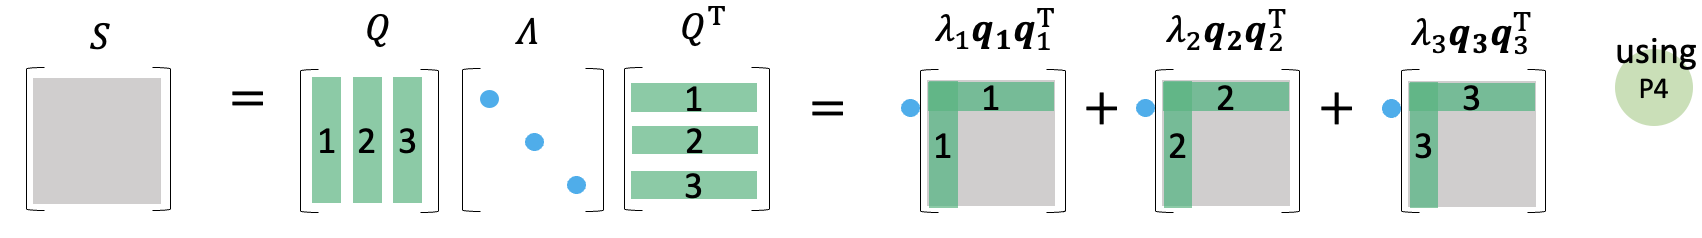
\includegraphics[keepaspectratio, width=\linewidth]{EVD.png}
  \caption{$S=Q \Lambda Q^\mathbf{T}$}
\end{figure}

A symmetric matrix $S$ is diagonalized into $\Lambda$  by an orthogonal matrix $Q$
and its transpose. And it is broken down into a combination of rank 1 projection matrices $P=qq^\mathbf{T}$.
This the spectral theorem.

Note that Pattern 4 (P4) is working for the decomposition.

\begin{gather*}
  S=S^\mathbf{T} = \lambda_1 P_1 + \lambda_2 P_2 + \lambda_3 P_3\\
  QQ^\mathbf{T} = P_1 + P_2 + P_3 = I \\
  P_1 P_2 = P_2 P_3 = P_3 P_1 = O\\
  P_1^2 =P_1=P_1^\mathbf{T}, \quad P_2^2=P_2=P_2^\mathbf{T}, \quad P_3^2=P_3=P_3^\mathbf{T}
\end{gather*}

\clearpage

\subsection{$\boldsymbol{A=U \Sigma V^\mathbf{T}}$}

All matrices including rectangular ones have a singular value decomposition (SVD).

$A=U \Sigma V^\mathbf{T}$ has the singular vectors of $A$ in $U$ and $V$.
And its singular values in $\Lambda$.

\begin{itemize}
  \item Sec.7.1 (p.259) Singular Values and Singular Vecrtors
\end{itemize}


\begin{figure}[H]
  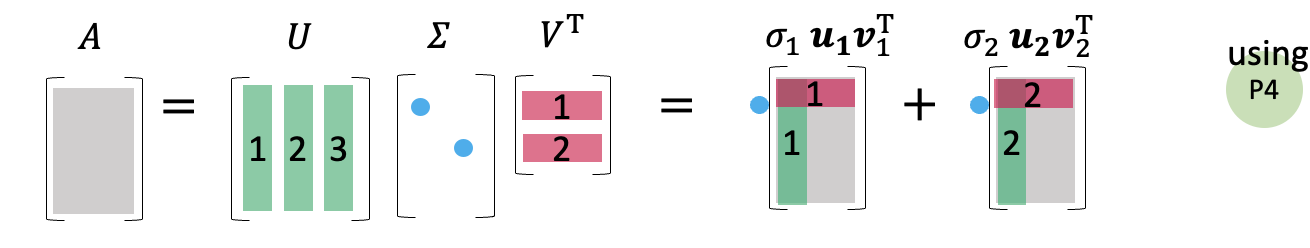
\includegraphics[keepaspectratio, width=\linewidth]{SVD.png}
  \caption{$A=U \Sigma V^\mathbf{T}$}
\end{figure}

You can find $V$ as an orthonormal basis of $\mathbb{R}^n$ (eigenvectors of $A^\mathbf{T}A$),
and $U$ as an orthonormal basis of $\mathbb{R}^m$ (eigenvectors of $AA^\mathbf{T}$).
Together they diagonalize $A$ into $\Sigma$.
This is also expressed as a combination of rank 1 matrices.

\begin{align*}
  A = U \Sigma V^\mathbf{T} =
  \begin{bmatrix}
    | & | & |\\
    \bm{u}_1 & \bm{u}_2 & \bm{u}_3\\
    | & | & |
  \end{bmatrix}
  \begin{bmatrix}
    \sigma_1 \\
           & \sigma_2 \\
           & &
  \end{bmatrix}
  \begin{bmatrix}
  - \bm{v}_1^\mathbf{T} -\\
  - \bm{v}_2^\mathbf{T} -
  \end{bmatrix}
  & =
  \sigma_1 \begin{bmatrix}
    |\\
    \bm{u}_1\\
    |
  \end{bmatrix}
  \begin{bmatrix}
    - \bm{v}_1^\mathbf{T} - 
  \end{bmatrix}
  +
  \sigma_2 \begin{bmatrix}
  |\\
  \bm{u}_2\\
  |
  \end{bmatrix}
  \begin{bmatrix}
  - \bm{v}_2^\mathbf{T} -
  \end{bmatrix} \\
& = \sigma_1 \bm{u}_1 \bm{v}_1^\mathbf{T} + \sigma_2 \bm{u}_2 \bm{v}_2^\mathbf{T}
\end{align*}

Note that:

\begin{align*}
  U U^\mathbf{T} &= I_m \\
  V V^\mathbf{T} &= I_n
\end{align*}

See Pattern 4 (P4) for the graphic notation.

\section*{Conclusion and Acknowledgements}

I presented systematic visualizations of matrix/vector multiplication and
their application to the Five Matrix Factorizations. I hope you
enjoyed them and will use them
in your understanding of Linear Algebra.

Ashley Fernandes helped me with beautifying this paper in typesetting
and made it much more consistent and professional.

To conclude this paper, I'd like to thank Prof. Gilbert Strang for
publishing ``Linear Algebra for Everyone". It guides us
through a new vision to these beautiful landscapes in Linear Algebra.
Everyone can reach a fundamental understanding of its underlying ideas
in a practical manner that introduces us to contemporary and also
traditional data science and machine learning. An important part of the matrix world.


\end{document}